\documentclass[12pt]{article}

\usepackage[affil-it]{authblk}
\usepackage[shortlabels]{enumitem}
\usepackage[utf8]{inputenc}
\usepackage{algorithm, algorithmicx, algpseudocode}
\usepackage{amsfonts, amsthm, amsmath, amssymb}
\usepackage{color}
\usepackage{cancel, textcomp}
\usepackage{enumerate}
\usepackage[mathscr]{euscript}
\usepackage{fancyhdr, fancyvrb}
\usepackage{fullpage}
\usepackage[left=0.5in,right=0.5in,headsep=0.5in,headheight=0.5in]{geometry}
\usepackage{graphicx}
\usepackage{hyperref}
\usepackage{latexsym}
\usepackage{mathtools}
\usepackage{minted}
\usepackage{times}
\usepackage{xcolor}
\usepackage{physics}
\usepackage{tikz-cd}
\usepackage[warnunknown, fasterrors, mathletters]{ucs}
\usepackage[nointegrals]{wasysym}

\newcommand{\hw}[2]{
    \noindent
    \begin{center}
        \framebox{
            \vbox{
                \hbox to 7in { {\bf MATH 470: Communications and Cryptography } \hfill  }
                \vspace{2mm}
                \hbox to 7in { {\Large \hfill Homework #1\hfill} }
                \vspace{2mm}
                \hbox to 7in { {\it Due date: #2 \hfill Name: Huy Lai } }
            }
        }
    \end{center}
    \vspace*{4mm}
}

\newcounter{prob}
\setcounter{prob}{0}
\newcounter{subprob}
\setcounter{subprob}{0}

\newcommand{\problem}{\setcounter{subprob}{0}\stepcounter{prob}{\noindent\textbf{Problem \theprob.}}\ }
\newcommand{\subproblem}{\stepcounter{subprob}{\noindent\textbf{Subproblem \thesubprob.}}\ }
\newcommand{\solution}{\noindent\textbf{Solution:}\newline}

\newcommand{\babc}{\begin{enumerate}[a)]}
\newcommand{\eabc}{\end{enumerate}}

\everymath{\displaystyle}

\setlength{\parskip}{.1in}
\setlength{\headheight}{15pt}
\setlength{\topmargin}{0pt}

\fancyhf{}
\pagestyle{fancy}
\lhead{MATH 470: Communications and Cryptography}
\rhead{Texas A\&M University}
\cfoot{\thepage}


\begin{document}
\hw{3}{13 September 2023}

\problem Let $p=587$ and numbers $a=345$, compute $a^{-1}\mod{p}$ in two
ways:

\begin{enumerate}[(i)]
    \item Use the extended Euclidean algorithm.
    \item Use the fast power algorithm and Fermat’s little theorem.
\end{enumerate}

\solution Using the Extended Euclidean Algorithm

\noindent
\begin{tabular}{|c|c|c|c|}
    \hline
    $q$ & $r$   & $u$   & $v$   \\
    \hline
        & $587$ & $0$   & $1$   \\
        & $345$ & $1$   & $0$   \\
    $1$ & $242$ & $-1$  & $1$   \\
    $1$ & $103$ & $2$   & $-1$  \\
    $2$ & $36$  & $-5$  & $3$   \\
    $2$ & $31$  & $12$  & $-7$  \\
    $1$ & $5$   & $-17$ & $10$  \\
    $6$ & $1$   & $114$ & $-67$ \\
    $5$ & $0$   & $u$   & $v$   \\
    \hline
\end{tabular}

\noindent
According to the EEA, the integers $(u,v)=(114,-67)$.\\
$354(114)+587(-67)=1$\\
$345^{-1}\equiv114\mod{587}$

\newpage
\noindent
Using the fast power algorithm and Fermat's Little Theorem.

\noindent
Fermat's Little Theorem states
\[a^{p-1}\equiv 1\mod{p}\]
Multiplying both sides of this by $a^{-1}$ results in
\[a^{p-2}\equiv a^{-1}\mod{p}\]
Therefore,
\[a^{-1}\equiv a^{p-2}\mod{p}\]

\noindent
$p-2=585_{10}=1001001001_2$

\begin{flalign*}
    a^{2^0} & \equiv a^{1}   \equiv 345\mod{p} & \\
    a^{2^1} & \equiv a^{2}   \equiv 451\mod{p} & \\
    a^{2^2} & \equiv a^{4}   \equiv 299\mod{p} & \\
    a^{2^3} & \equiv a^{8}   \equiv 177\mod{p} & \\
    a^{2^4} & \equiv a^{16}  \equiv 218\mod{p} & \\
    a^{2^5} & \equiv a^{32}  \equiv 564\mod{p} & \\
    a^{2^6} & \equiv a^{64}  \equiv 529\mod{p} & \\
    a^{2^7} & \equiv a^{128} \equiv 429\mod{p} & \\
    a^{2^8} & \equiv a^{256} \equiv 310\mod{p} & \\
    a^{2^9} & \equiv a^{512} \equiv 419\mod{p} & \\
\end{flalign*}
$345^{585}=345^{2^9+2^6+2^3+2^0}\equiv419\cdot529\cdot177\cdot345\equiv114\mod{587}$\\
$345^{-1}\equiv114\mod{587}$

\newpage
\problem Let $p$ be a prime and let $q$ be a prime that divides $p-1$. Let $a\in\mathbb{F}_p^*$ and let $b=a^{\frac{p-1}{q}}$. Prove that either $b=1$ or else $b$ has order $q$.

\solution The proof is as follows.
\begin{proof}
    Let $k$ be the order of $b$.\\
    Raising the definition of $b$ to the power of $q$ will result in
    \[b^q=a^{p-1}\]
    By Fermat's Little Theorem, $b^q\equiv a^{p-1}\equiv 1\mod{p}$\\
    By Proposition 1.29 in the Textbook, $k\mid q$. Since $q$ is prime, then $k=1$ or $k=q$.\\
    As a result either $b$ has order $q$, or it has order 1.
\end{proof}

\problem Let $p$ be a prime such that $q=\frac{1}{2}(p-1)$ is also prime. Suppose that $g$ is an integer satisfying
\[g\not\equiv 0\mod{p},g\not\equiv\pm1\mod{p},g^q\not\equiv1\mod{p}\]
Prove that $g$ is a primitive root modulo $p$.

\solution The proof is as follows.
\begin{proof}
    Let $k$ be the order of $g$. Then by proposition, $k\mid (p-1)$.\\
    Since $p-1=2q$ with $q$ prime, this means that
    \[k=1\text{ or } k=2 \text{ or } k=q \text{ or } k=2q\]

    \noindent
    If $k=1$, that means that $g=g^1\equiv1\mod{p}$. Therefore $k\neq1$\\
    If $k=2$, then $g^2\equiv1\mod{p}$. This implies that $g\equiv1\mod{p}$. Because $\pm1\in(\mathbb{Z}/p\mathbb{Z})^*$. Therefore $k\neq2$\\
    Since $g^q\not\equiv1\mod{p}$, then $k\neq q$.\\
    As a result $k=2q\Rightarrow k=p-1$.\\
    With this, the order of $g$ is $p-1$, this satisfies the definition of a primitive root.\\
    Therefore, $g$ is a primitive root modulo $p$.
\end{proof}

\newpage
\problem Let $p$ be an odd prime number and let $b$ be an integer with $p\nmid b$. Prove that either $b$ has two square roots modulo $p$ or else $b$ has no square roots modulo $p$. In other words, prove that the congruence
\[X^2\equiv b\mod{p}\]
has either two solutions or no solutions in $\mathbb{Z}/p\mathbb{Z}$. (What happens for $p=2$? What happens if $p\mid b$?)

\solution The proof is as follows.
\begin{proof}
    Let $a_1,a_2$ be solutions to the congruency.\\
    Then by proposition of modulo, $p\mid\left(a_1^2-b\right)$ and $p\mid\left(a_2^2-b\right)$.\\
    By proposition of divisibility, $p\mid\left[\left(a_1^2-b\right)-\left(a_2^2-b\right)\right]$\\
    This can be rewritten as
    \[p\mid(a_1-a_2)(a_1+a_2)\]

    \noindent
    From this, $p$ must divide either $a_1-a_2$ or $a_1+a_2$.\\
    If $p\mid(a_1-a_2)$, then $a_1\equiv a_2\mod{p}$. If $p\mid(a_1+a_2)$, then $a_1\equiv-a_2\mod{p}$.\\
    As a result, there are a most two solutions.

    \noindent
    We prove that one solution is not possible by contradiction.\\
    Let $a$ be the solution to the congruency.\\
    Then, $a^2\equiv b\mod{p}$.\\
    We can generate another unique solution by completing the square as follows
    \[p^2+2ap+a^2\equiv b\mod{p}\]
    This gives that $(p+a)^2\equiv b\mod{p}$. However, $p+a\not=a$.\\
    Therefore, if one solution exists, another can be found.\\
    This proves that there are zero or two solutions.
\end{proof}

\clearpage
\problem Problem 5

\subproblem Let $p=13$ and let $g=2$. Note that $p$ is prime and that $g$ is a primitive root modulo $p$. Make a list of the powers of $g$ and their orders modulo $p$ (i.e., for each $a\in\{1,2,3,\cdots,12\}$, write down $g^a \mod{p}$ and the order of $g^a \mod{p}$). What are all the primitive roots modulo $p$? Compute $\phi(p-1)$, where $\phi$ is the Euler’s totient function.

\solution
\begin{tabular}{|c|c|c|}
    \hline
    $a$  & $2^a \mod{13}$ & Order \\
    \hline
    $1$  & $2$            & $12$  \\
    $2$  & $4$            & $6$   \\
    $3$  & $8$            & $4$   \\
    $4$  & $3$            & $3$   \\
    $5$  & $6$            & $12$  \\
    $6$  & $12$           & $2$   \\
    $7$  & $11$           & $12$  \\
    $8$  & $9$            & $3$   \\
    $9$  & $5$            & $4$   \\
    $10$ & $10$           & $6$   \\
    $11$ & $7$            & $12$  \\
    $12$ & $1$            & $1$   \\
    \hline
\end{tabular}

\noindent
The primitive roots modulo $p$ are:
$2,6,11,7$ which are $g^1,g^5,g^7,g^{11}$
$\phi(n-1)=\phi(12)=4$

\clearpage
\subproblem Let $p$ be a prime, let $g$ be a primitive root modulo $p$, and let $a$ be an integer. Prove that the order of $g^a\mod{p}$ is exactly $\frac{p-1}{\gcd(a,p-1)}$. Explain why this implies that the number of primitive roots modulo $p$ is exactly $\phi(p-1)$, assuming that a primitive root $g$ modulo $p$ exists. (Looking over your work in part (a) may help you gain some intuition).

\solution The proof is as follows
\begin{proof}
    Let $n$ by the order of $g^a\mod{p}$.\\
    $gcd(a,p-1)\mid a\rightarrow\exists x\in\mathbb{Z}$ such that $a=x\gcd(a,p-1)$ by definition of divisibility.
    \[\left(g^a\right)^{\frac{p-1}{\gcd(a,p-1)}}=\left(g^{x\cdot\gcd(a,p-1)}\right)^{\frac{p-1}{\gcd(a,p-1)}}=g^{x(p-1)}=\left(g^{(p-1)}\right)^x\equiv1^x\equiv1\mod{p}\]
    The second congruence is due to Fermat's Little Theorem.\\
    This implies that $n\leq\frac{p-1}{\gcd(a,p-1)}$.

    \noindent
    By proposition, $n\mid(p-1)$. Therefore $\exists y\in\mathbb{Z}$ such that $p-1=ny$.\\
    By definition of $n$, $g^{an}=(g^a)^n\equiv1\mod{p}$.\\
    By proposition, $p-1\mid an=\frac{a(p-1)}{y}$ this implies that $\frac{a}{y}\in\mathbb{Z}$ which further implies that $y\mid a$.\\
    Clearly $y\mid (p-1)$ by its definition. Therefore, $y$ is a common divisor of $a$ and $p-1$ which implies that $y\leq\gcd(a,p-1)$.
    Since $n=\frac{p-1}{y}\geq\frac{p-1}{\gcd(a,p-1)}$.

    \noindent
    We have shown that $n\leq\frac{p-1}{\gcd(a,p-1)}$ and that $n\geq\frac{p-1}{\gcd(a,p-1)}$.\\
    Therefore the order of $g^a\mod{p}$ is $n=\frac{p-1}{\gcd(a,p-1)}$
\end{proof}

\clearpage
\problem You may assume that the following integers $p$ and $q$ are primes:
\begin{flalign*}
    p & = 1234567890123456789012345678901234567890123456789012345678901234567890123459287 \\
    q & = 617283945061728394506172839450617283945061728394506172839450617283945061729643  \\
\end{flalign*}
Also note that $p=2q+1$. Find the smallest positive integer $g$ that is a primitive root modulo $p$.

\solution
\inputminted{py}{proot.py}

\begin{figure}[!ht]
    \centering
    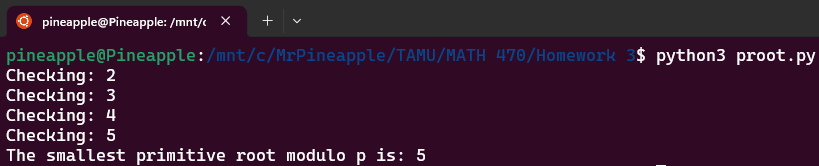
\includegraphics[width=0.9\textwidth]{Question 6.png}
    \caption{Output}
\end{figure}

\end{document}
